%%
%% This is file `S_article2.tex',
%% generated with the docstrip utility.

%% Utilisez la macro de langue appropriée.
\francais   
%ou
%%\anglais

\setcounter{figure}{0}
\renewcommand{\thefigure}{B\arabic{figure}}

\setcounter{table}{0}
\renewcommand{\thetable}{\arabic{chapter}.\arabic{table}}

\chapter{Supplementary material of Article~\ref{art:article2}}\label{supp:B}

\begin{figure}[h]
    \centering
    \includegraphics[width=\textwidth]{figures/S_article2/kin_kout_difference_strata.png}
    \caption{\textbf{Prediction errors of the absolute number of predators $k_{in}$ and prey
    $k_{out}$.} Species were ordered according to their total degree in their
    network. Networks were sorted into different groups based on their total number
    of species. In each panel, each dot corresponds to a single species within one
    of the networks whose total species count is within the specified range. The
    predicted joint degree sequences were obtained after sampling one realization of
    the joint degree distribution of maximum entropy for each network while keeping
    the total number of interactions
    constant.}
    \label{fig:kin_kout_diff_strata}
\end{figure}

\begin{figure}[h]
    \centering
    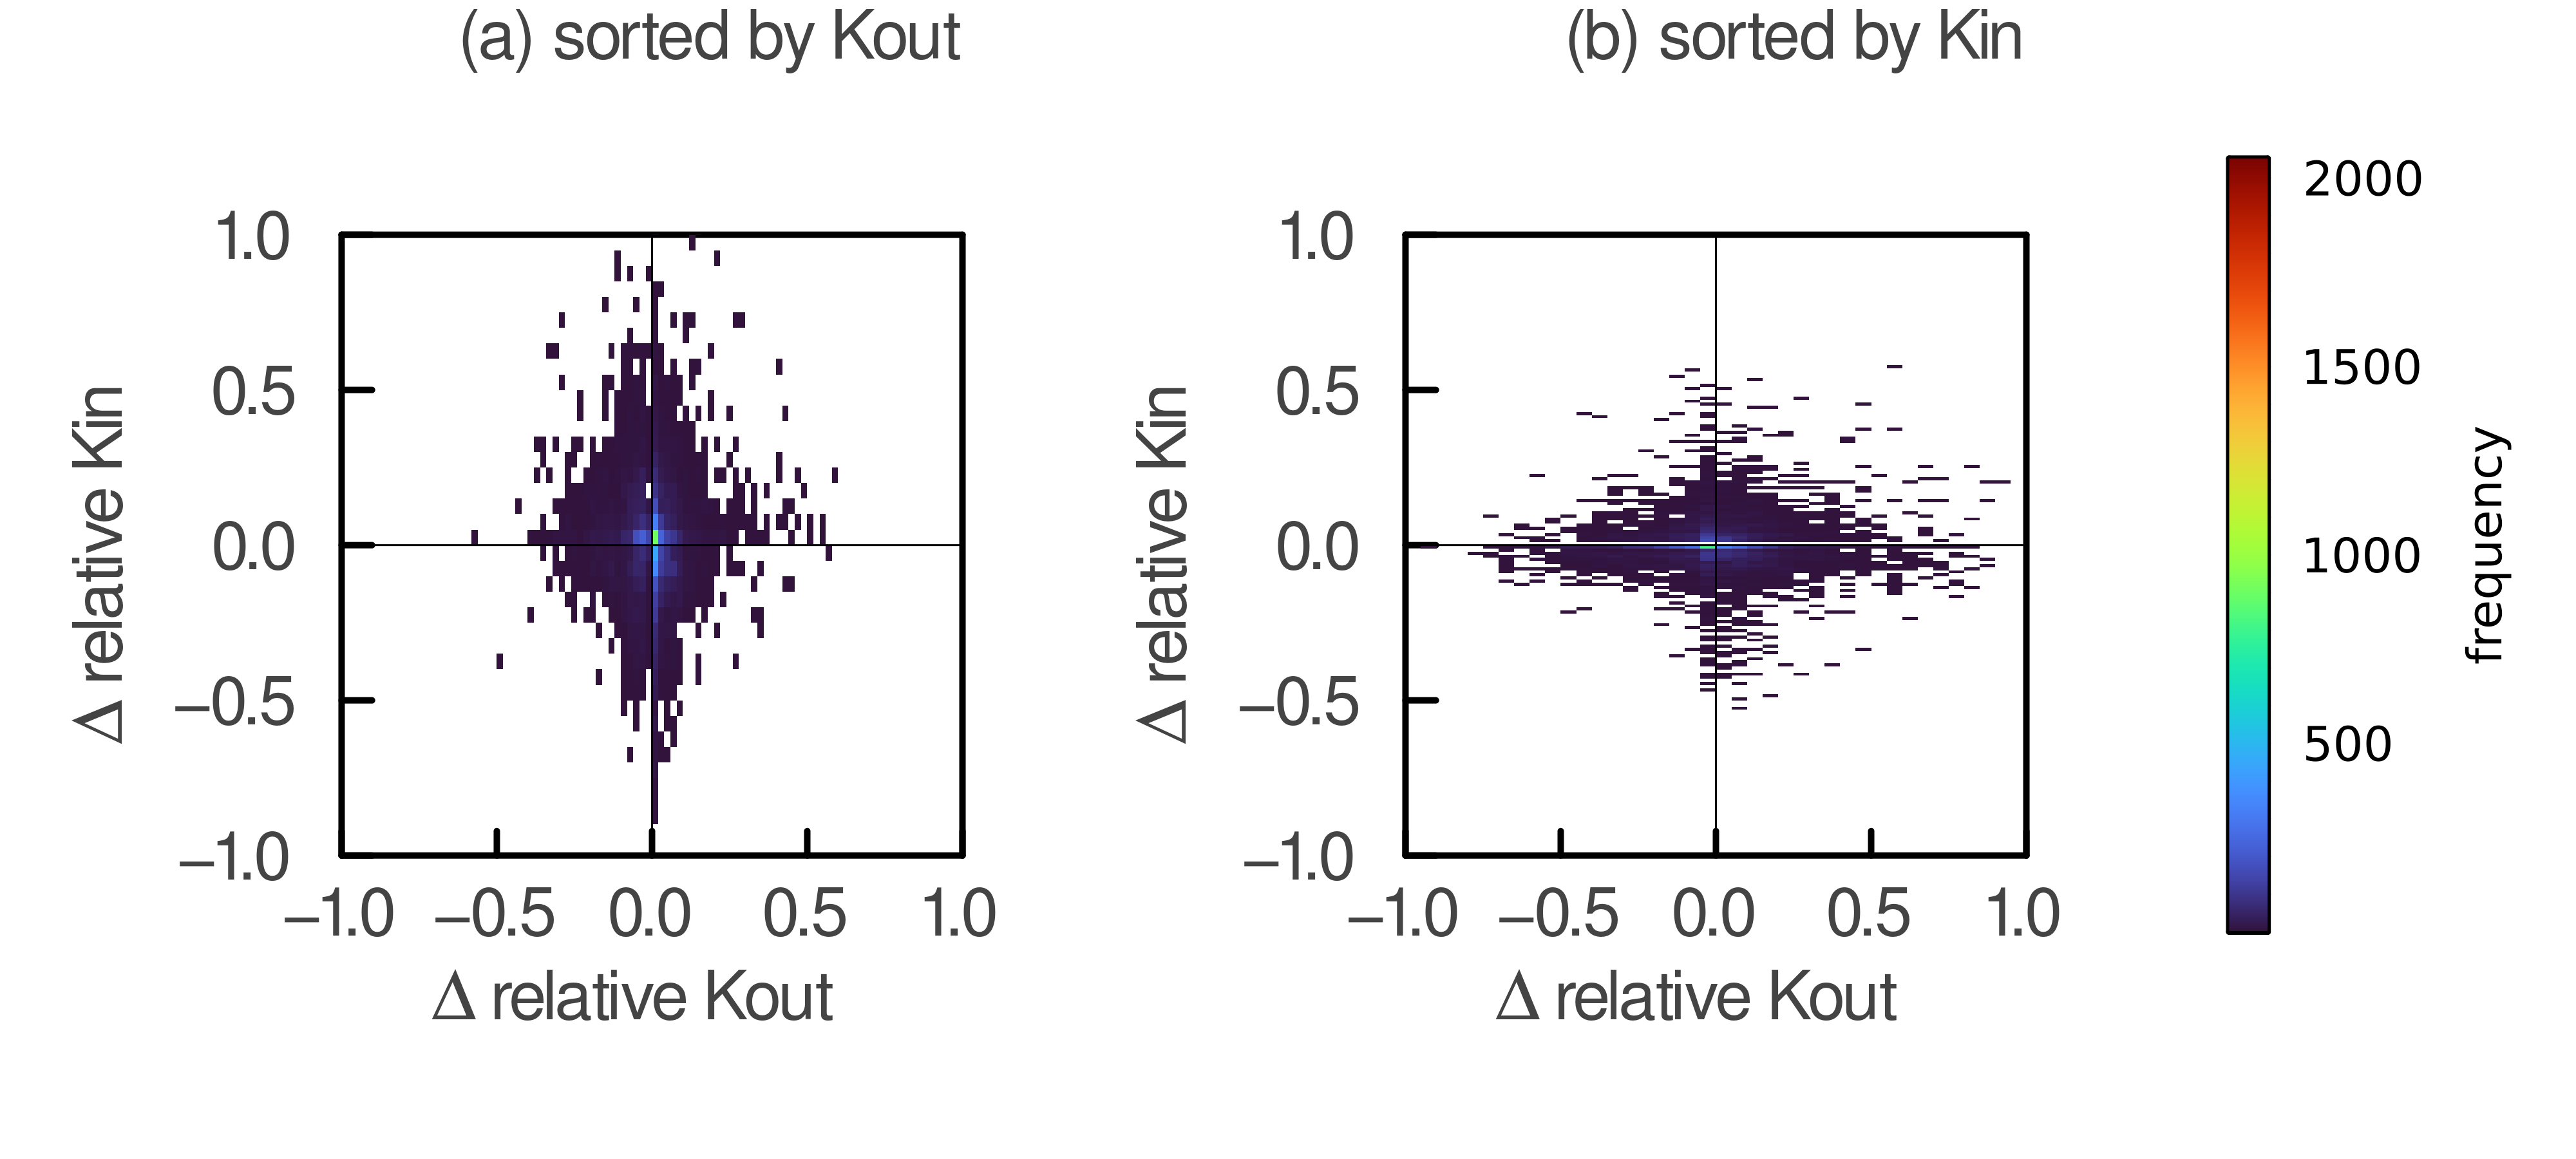
\includegraphics[width=\textwidth]{figures/S_article2/kin_kout_difference.png}
    \caption{\textbf{Prediction errors of the relative number of predators $k_{in}$ and prey
    $k_{out}$.} Species were ordered according to (a) their out-degree and (b)
    their in-degree. The predicted joint degree sequences were obtained after
    sampling one realization of the joint degree distribution of maximum entropy for
    each network while keeping the total number of interactions constant. Due to
    significant data overlap, all relationships are represented as 2D histograms.
    The color bar indicates the number of species that fall within each
    bin.}
    \label{fig:kin_kout_diff}
\end{figure}

\begin{figure}[h]
    \centering
    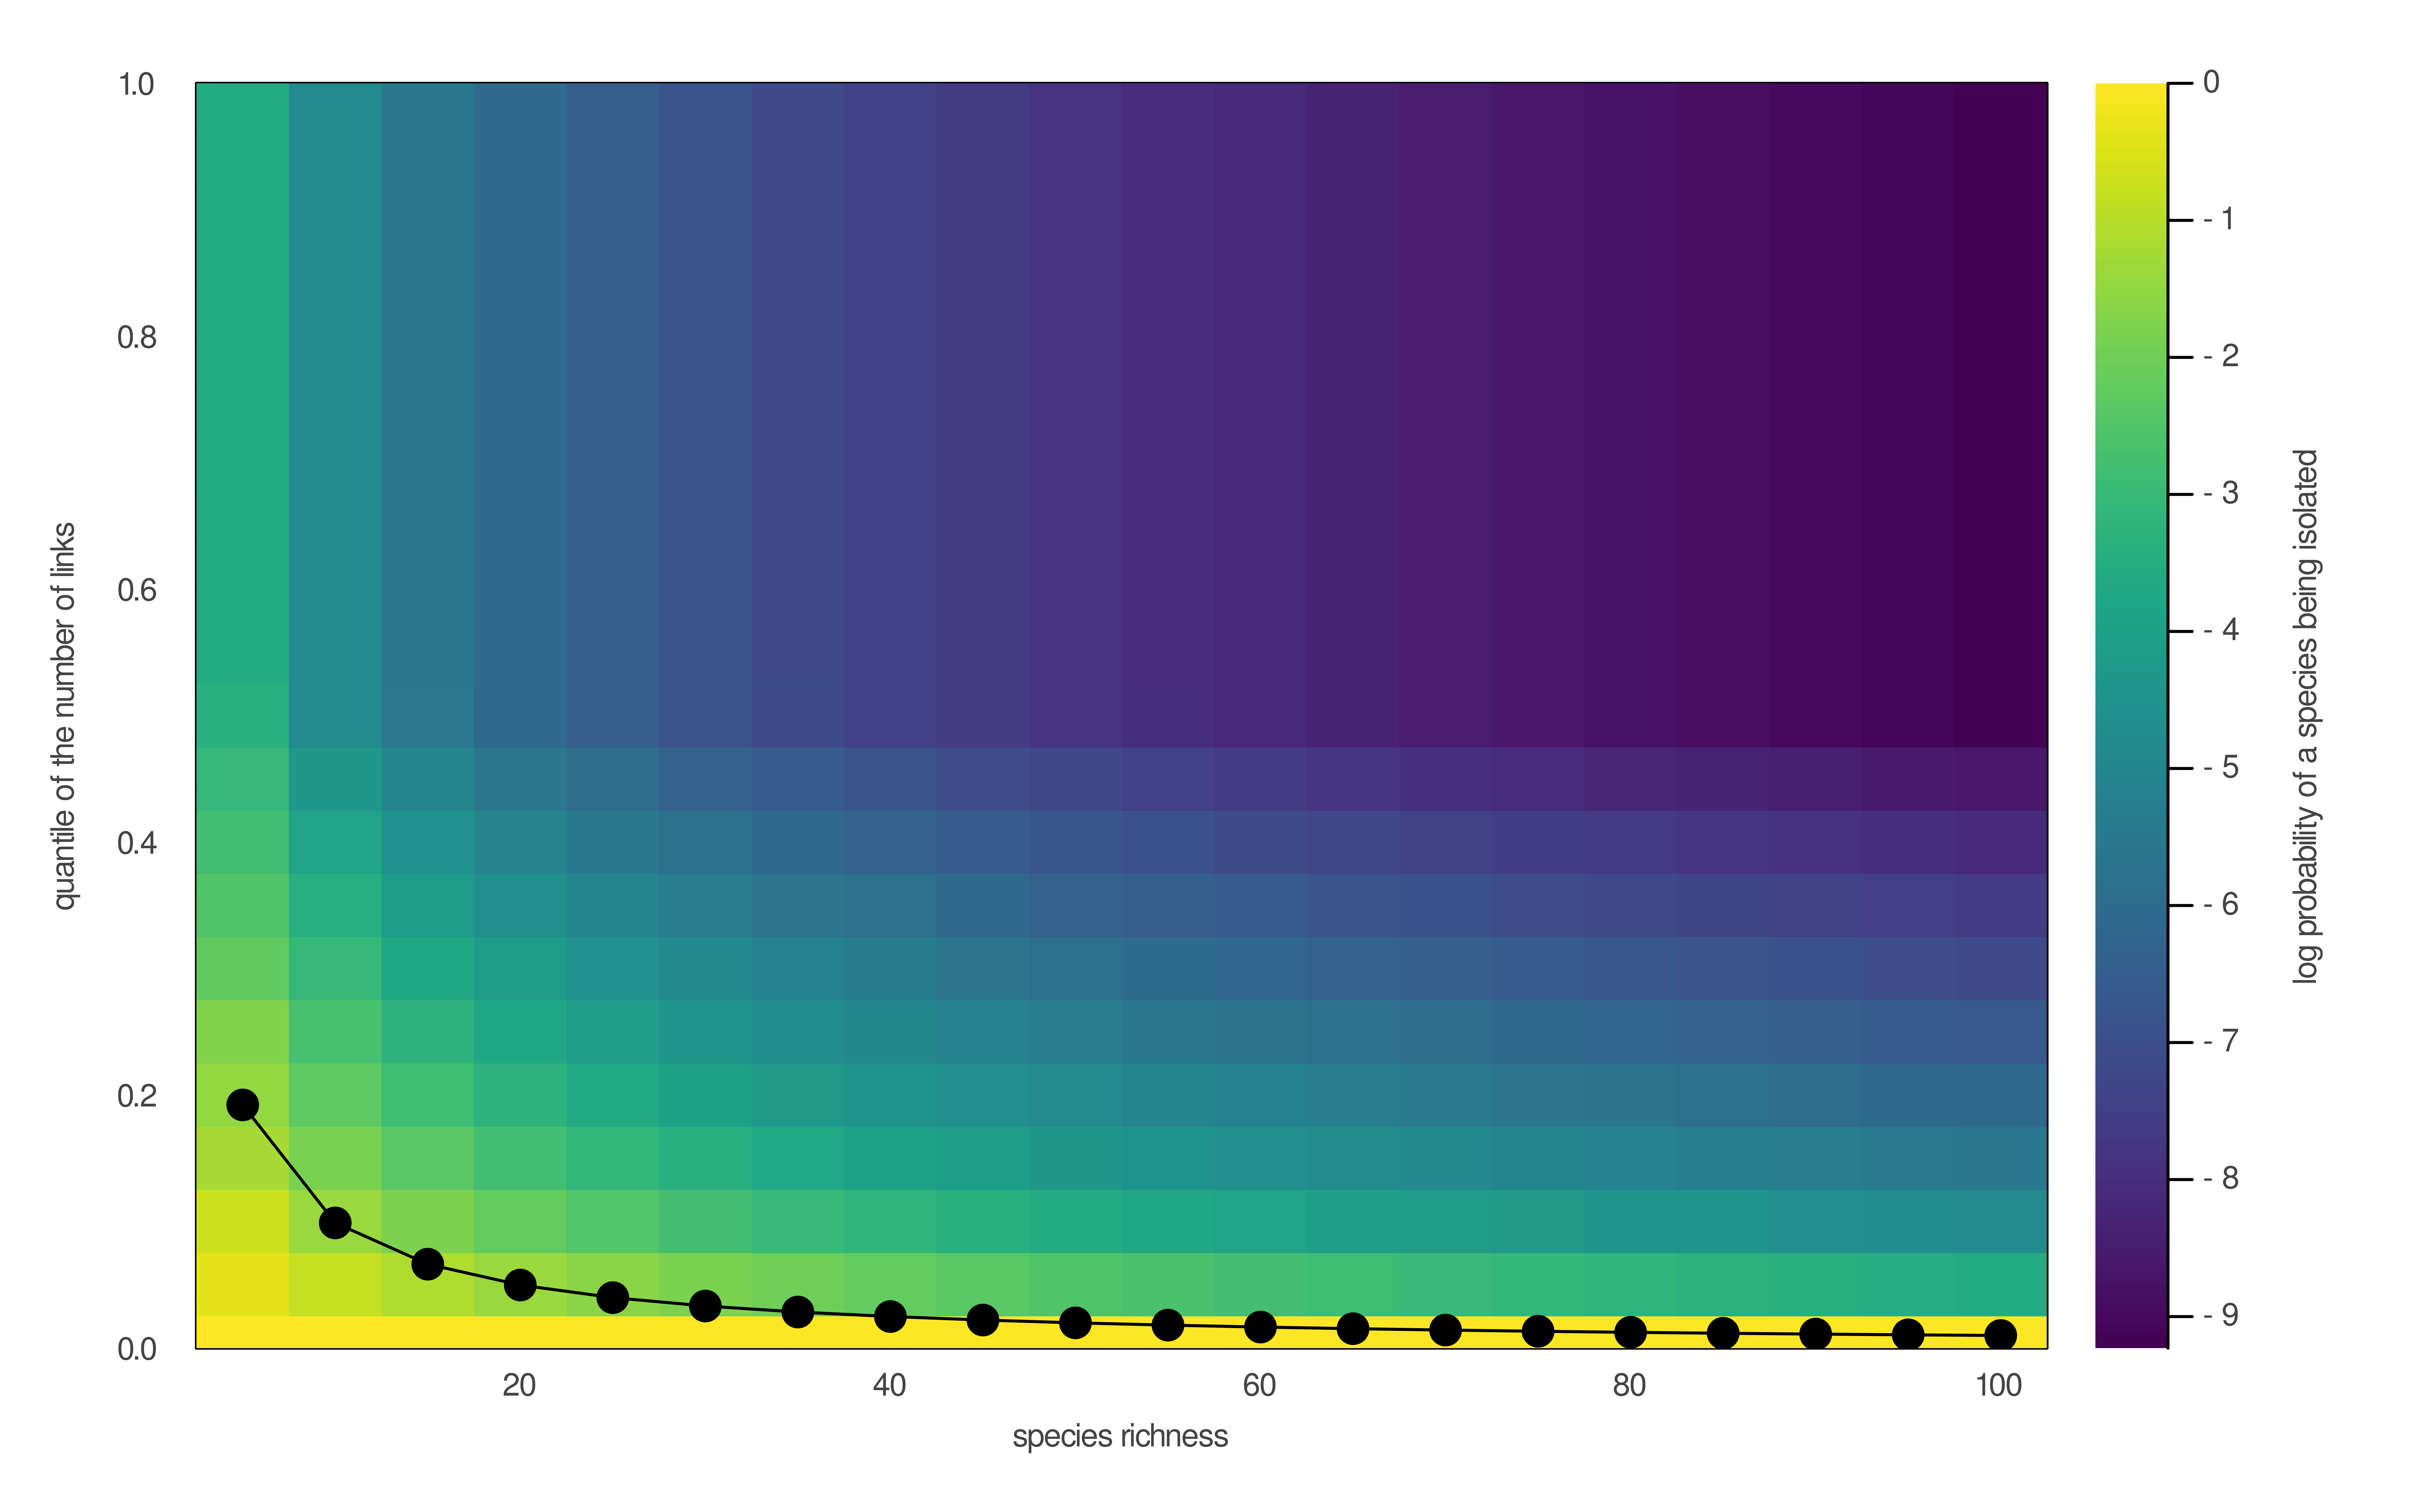
\includegraphics[width=\textwidth]{figures/S_article2/heatmap_disconnected.png}
    \caption{\textbf{Predicted probability that a species is isolated in its food web.} We
    derived many degree distributions of maximum entropy given a range of values of
    $S$ and $L$ and plotted the probability that a species has a degree $k$ of $0$
    (log-scale color bar). Species richness varies between $5$ and $100$ species, by
    increment of $5$ species. For each level of species richness, the numbers of
    interactions correspond to all 20-quantiles of the interval between $0$ and
    $S^2$. The black line marks the $S-1$ minimum number of interactions required to
    have no isolated species.}
    \label{fig:heatmap}
\end{figure}

\begin{figure}[h]
    \centering
    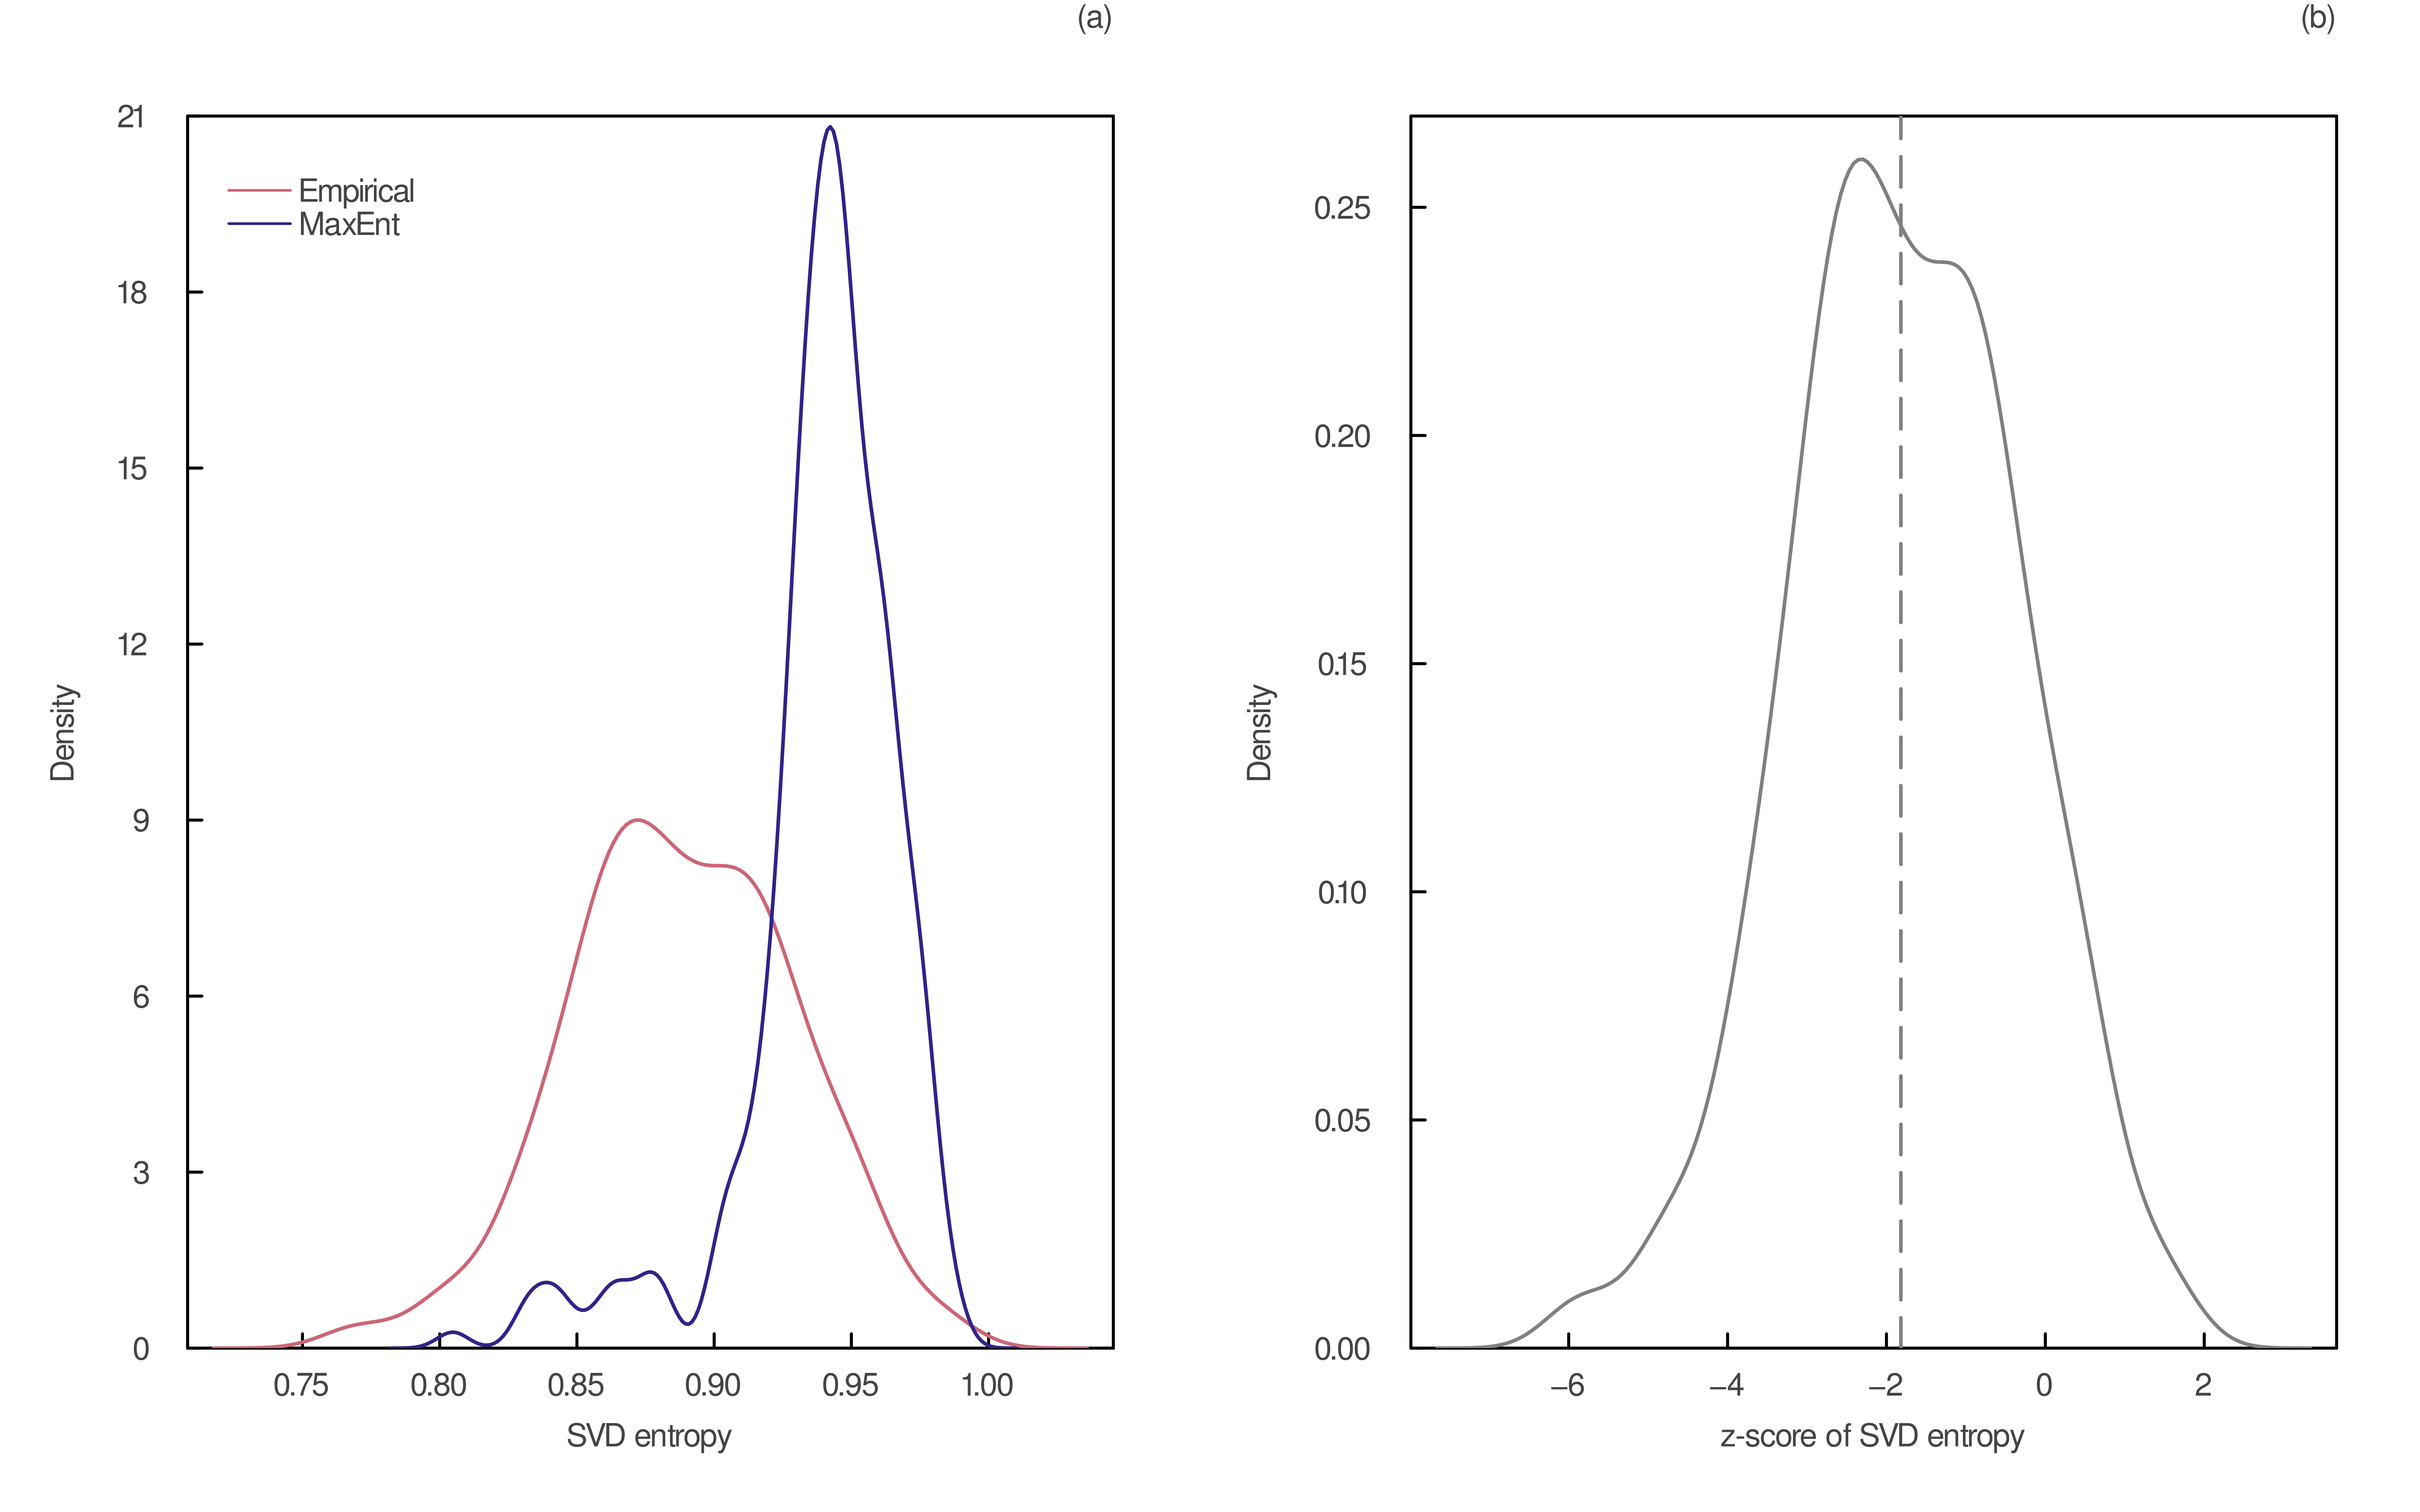
\includegraphics[width=\textwidth]{figures/S_article2/entropy_distribution.png}
    \caption{\textbf{SVD entropy of empirical and predicted food webs.} (a) Distribution of the
    SVD entropy of empirical and maximum entropy food webs. Maximum entropy networks
    were obtained using the type II heuristic MaxEnt model based on the joint degree
    sequence. (b) Distribution of z-scores of the SVD entropy of all empirical food
    webs. Z-scores were computed using the mean and standard deviation of the
    distribution of SVD entropy of MaxEnt food webs (type II heuristic MaxEnt
    model). The dashed line corresponds to the median
    z-score.}
    \label{fig:entropy_dist}
\end{figure}

\begin{figure}[h]
    \centering
    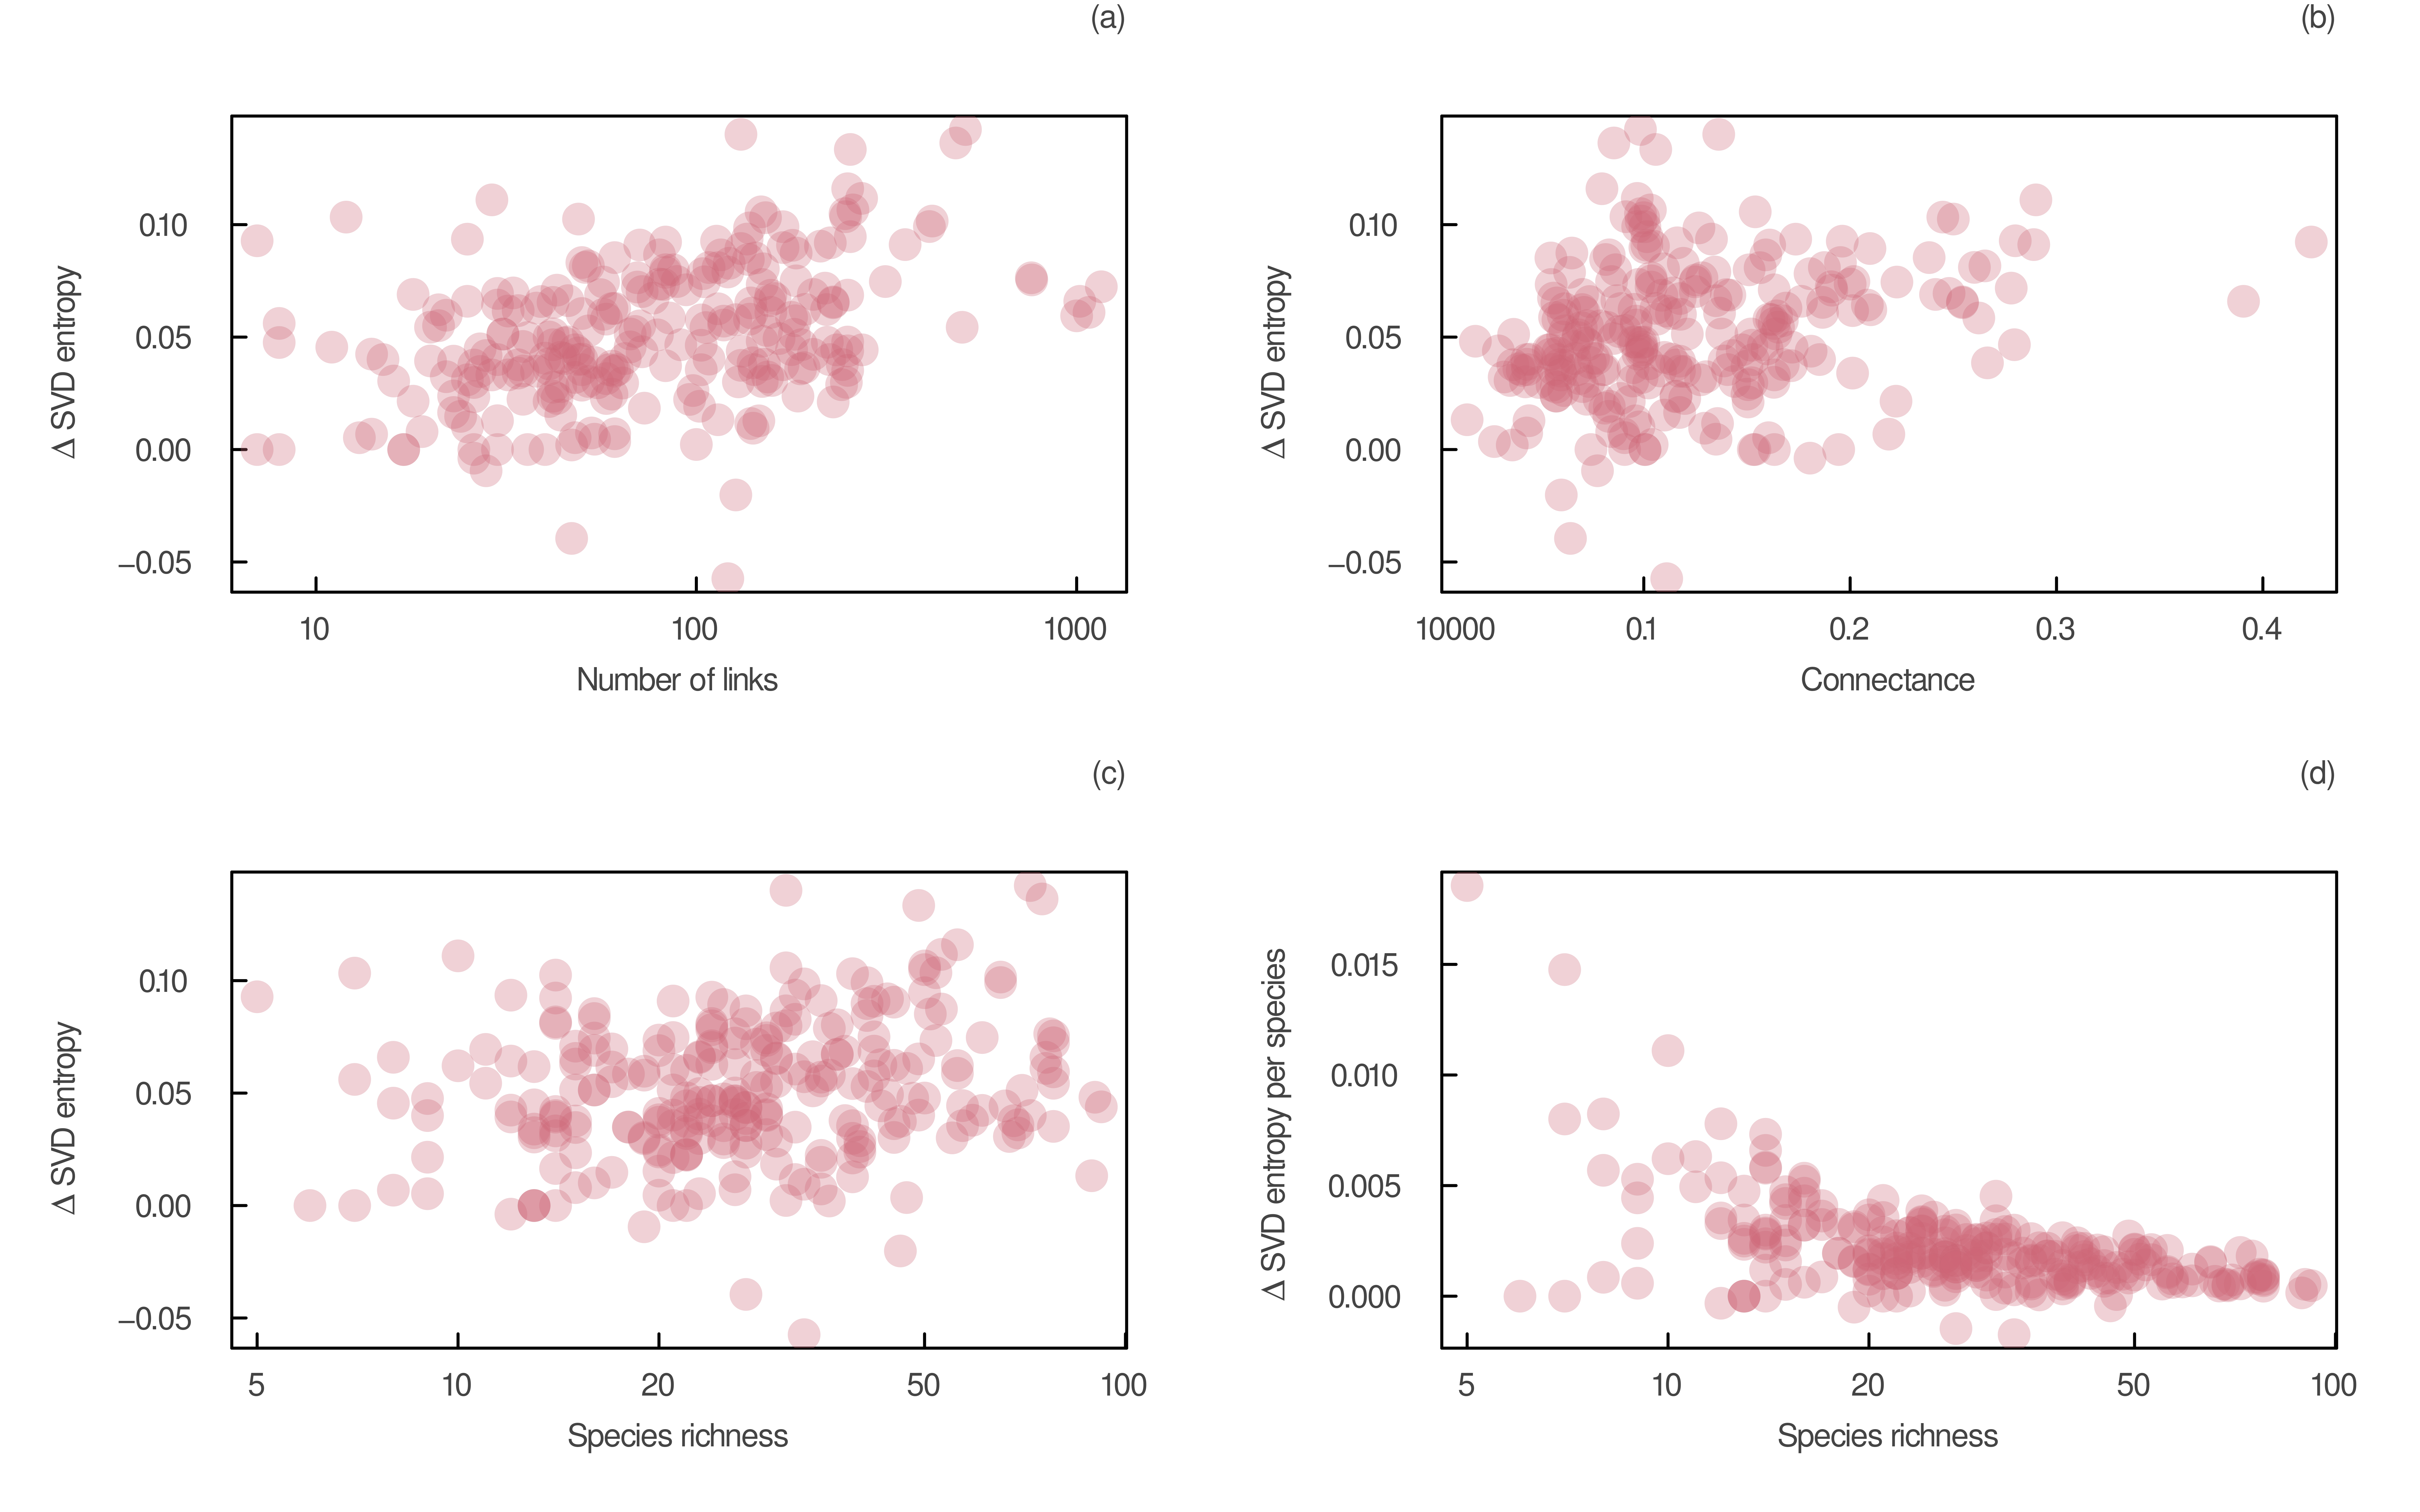
\includegraphics[width=\textwidth]{figures/S_article2/difference_entropy.png}
    \caption{\textbf{Prediction errors of SVD entropy.} Difference in SVD entropy between
    maximum entropy and empirical food webs as a function of (a) the number of
    interactions, (b) connectance, and (c) species richness. (d) Standardization of
    the difference in SVD entropy with respect to species richness as a function of
    species richness. The exponential decrease in the difference of SVD entropy per
    species with species richness offers a complementary perspective supporting the
    lack of relationship depicted in panel c. Maximum entropy networks were obtained
    using the type II heuristic MaxEnt model based on the joint degree
    sequence.}
    \label{fig:entropy_size}
\end{figure}

\begin{figure}[h]
    \centering
    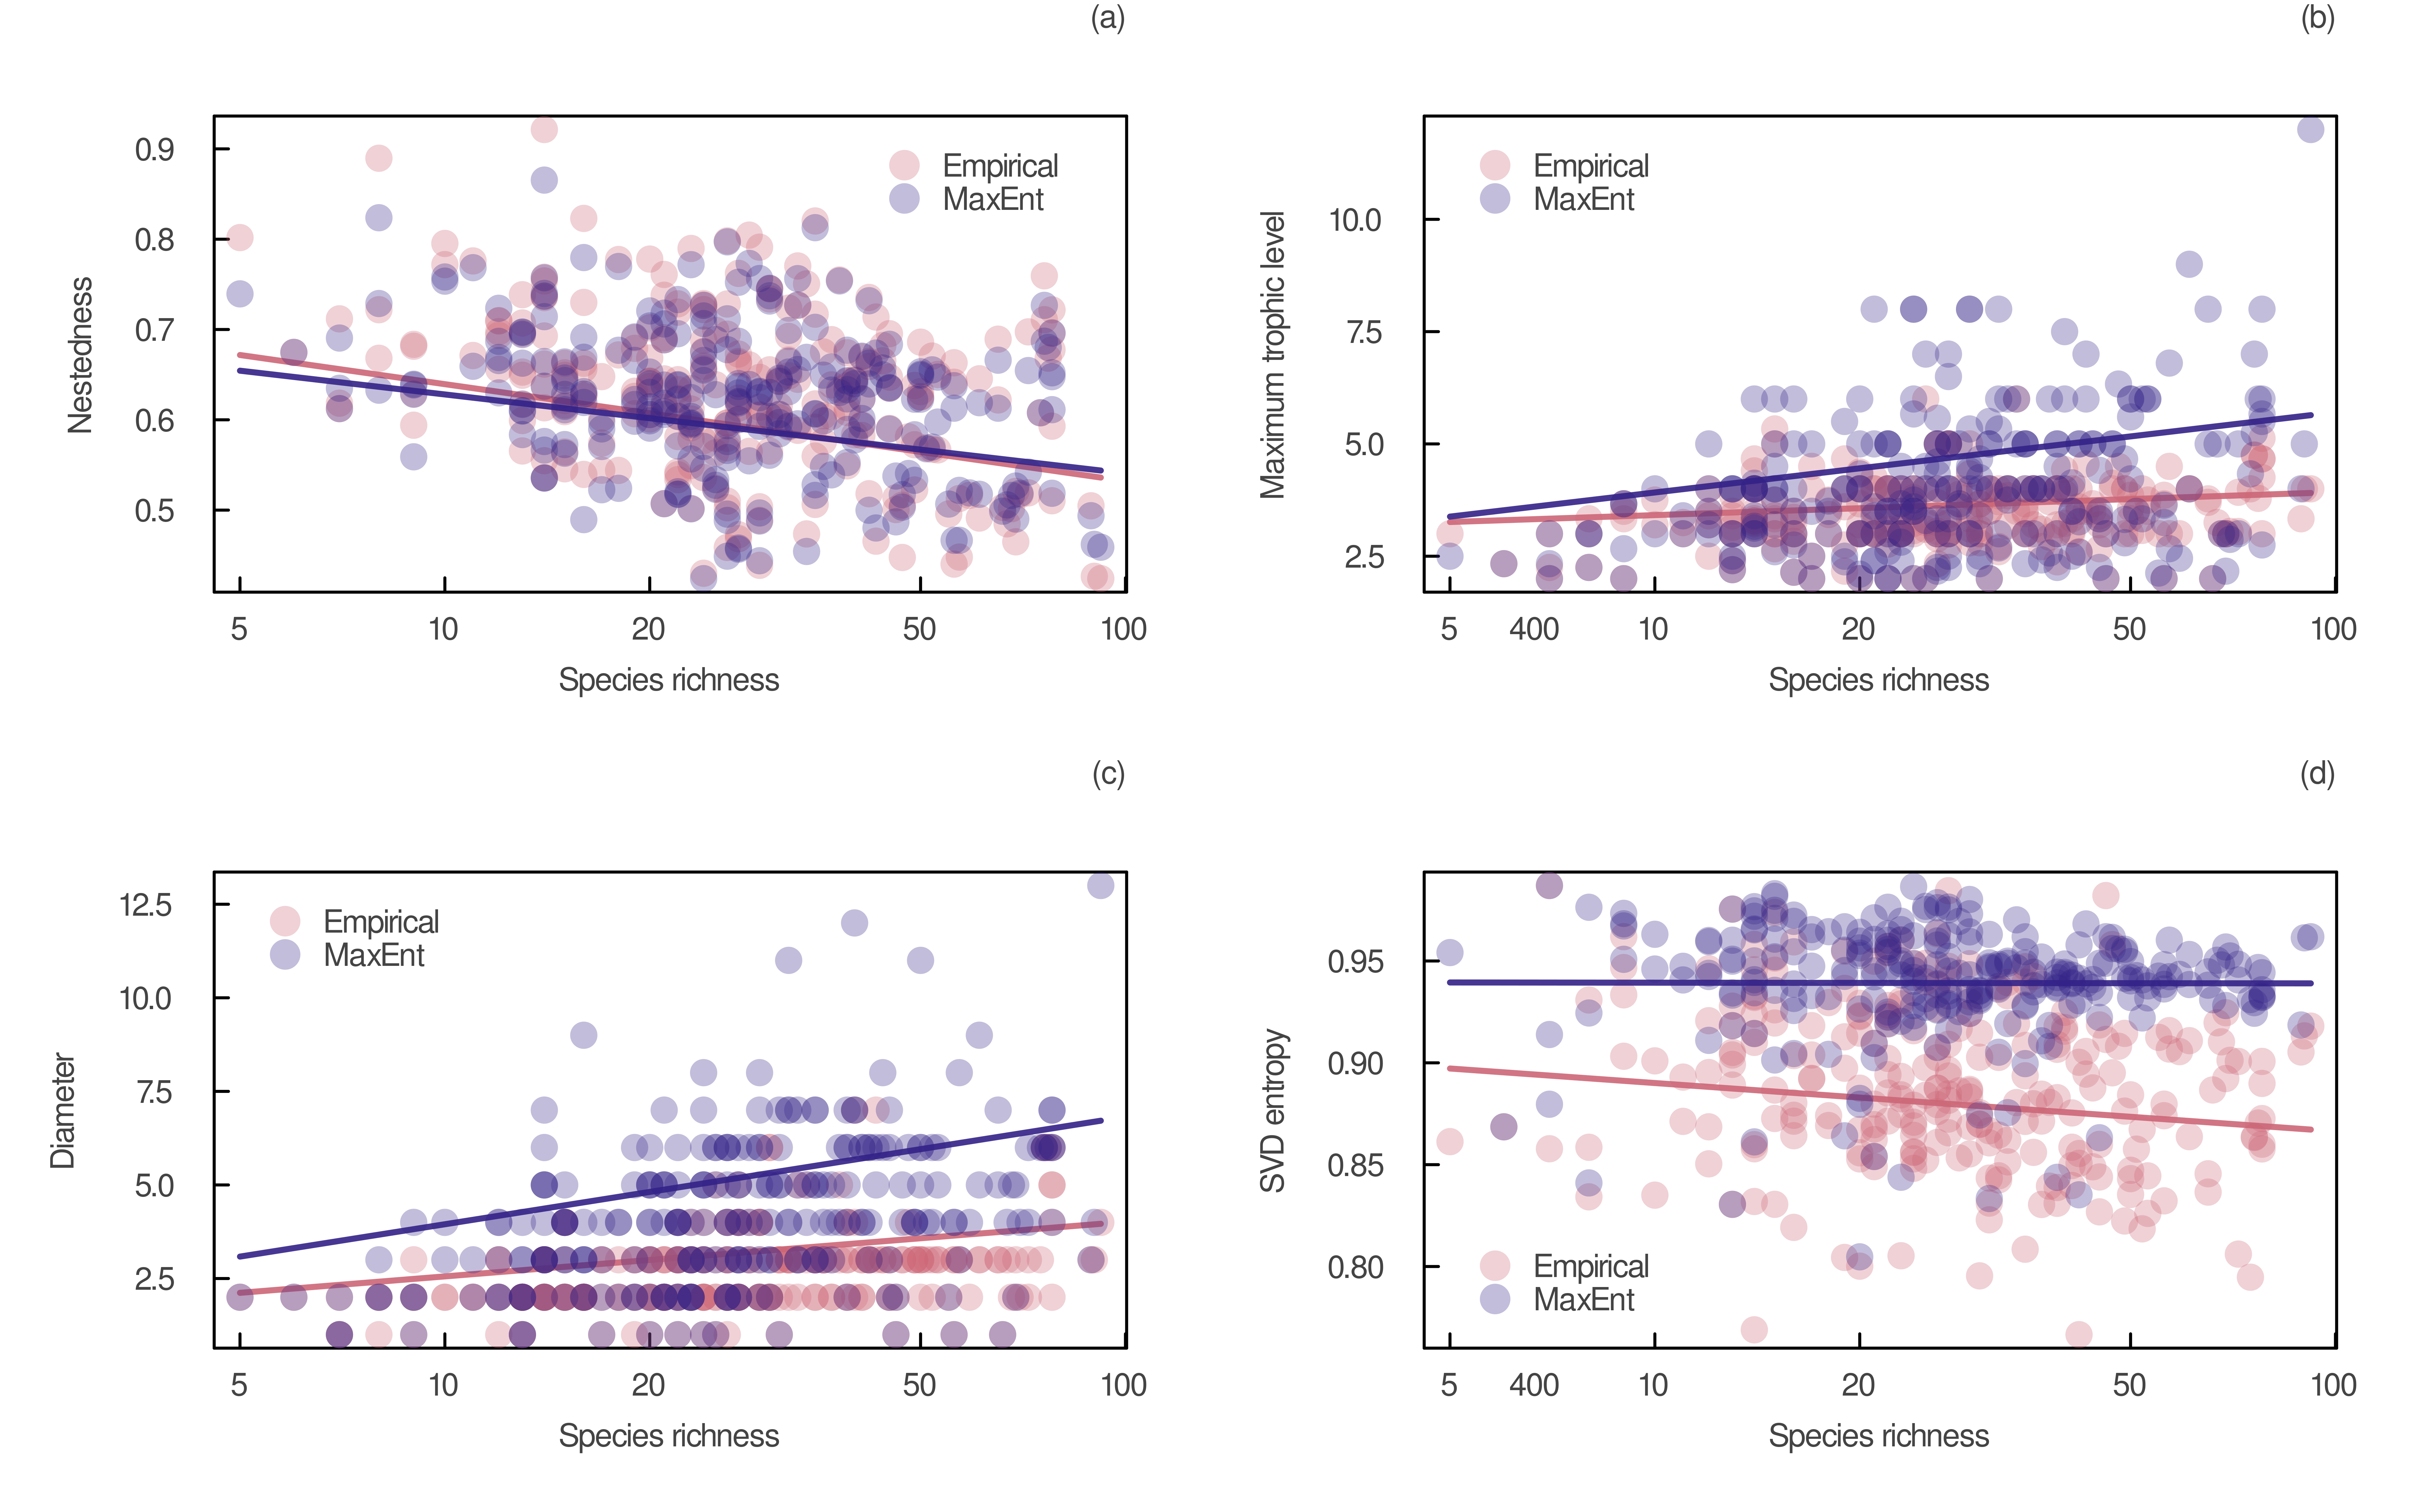
\includegraphics[width=\textwidth]{figures/S_article2/measures_richness.png}
    \caption{\textbf{Structure of empirical and maximum entropy food webs as a function of
    species richness.} Maximum entropy networks were obtained using the type II
    heuristic MaxEnt model based on the joint degree sequence. (a) Nestedness
    (estimated using the spectral radius of the adjacency matrix), (b) the maximum
    trophic level, (c) the network diameter, and (d) the SVD entropy were measured
    on these empirical and maximum entropy food webs and plotted against species
    richness. Regression lines are plotted in each
    panel.}
    \label{fig:measures_richness}
\end{figure}

\endinput
%%
%% End of file `S_article2.tex'.
